\chapter{\IfLanguageName{dutch}{literatuurstudie}{Introduction}}%
\label{ch:Literatuurstudie}

\subsection{Back-ups in het kader van bedrijfscontinuïteit en disaster recovery}
Bedrijfscontinuïteit verwijst naar de aanpak en procedures dat een bedrijf gebruikt om de voortgang van zijn werkzaamheden te bewaren, zelfs in het geval van incidenten. Deze incidenten kunnen variëren van relatief kleine problemen, zoals een gebroken netwerkverbinding, tot grote natuurrampen zoals een aardbevingen. Omdat er zoveel soorten incidenten kunnen gebeuren is het moeilijk om een oplossing te vinden die ervoor zorgt dat bedrijven in alle gevallen beschermt zijn. In plaats daarvan gebruiken bedrijven een mix van strategieën en technologieën om de continuïteit van hun processen te beschermen. De 2 belangrijkste concepten voor de bedrijfscontinuïteit zijn hoge beschikbaarheid en disaster recovery.

Hoge beschikbaarheid duidt op het feit dat een bedrijf zodanig is ingericht dat het kan blijven draaien, zelfs als bepaalde systemen of componenten uitvallen. Een voorbeeld hiervan zijn twee routers die zijn geconfigureerd in een actieve-passieve opstelling. In deze configuratie is één router de primaire router die al het inkomende en uitgaande verkeer verwerkt, terwijl de andere router als reserve werkt. In het geval dat de primaire router faalt door een hardwarestoringen of netwerkprobleem, dan neemt de tweede router automatisch de rol van de primaire router over, zonder dat dit merkbare impact heeft op de netwerkverbindingen van de organisatie. Hierdoor blijft de beschikbaarheid van het netwerk gegarandeerd en blijft de downtime laag \autocite{Zhu2015}.

Disaster recovery (DR) is een onderdeel van bedrijfscontinuïteit dat zich specifiek richt op het herstellen van bedrijfsactiviteiten na een incident zoals een cyberaanval of ernstige verstoring. Terwijl bedrijfscontinuïteit zich richt op bredere preventieve maatregelen om de continuïteit te waarborgen, focust disaster recovery zich juist op de praktische stappen en hulpmiddelen die nodig zijn om de organisatie na een verstoring weer snel operationeel te maken. Het doel van disaster recovery is om schade zoveel mogelijk te beperken en de normale gang van zaken zo snel mogelijk te herstellen .
 
Back-ups spelen een belangrijke rol voor de continuïteit van een bedrijf en zijn vaak de eerste stap bij het opstellen van een disaster recovery plan (DRP). Bij een optimale situatie is er na een incident geen data verloren en is alle data relatief snel terug beschikbaar. Indien een bedrijf geen back-ups heeft van de belangrijke data zal de data in het geval van een incident verloren raken. Zonder back-ups zal het ook een grotere uitdaging zijn voor het bedrijf om de normale bedrijfsactiviteiten terug uit te voeren. Een belangrijke doelstelling van een bedrijf is winst maken. In het geval van een incident waarbij de bedrijfsactiviteiten niet normaal kunnen verlopen zal deze doelstelling verhindert worden en zal er dus financieel verlies optreden. Bij specifieke bedreigingen, zoals ransomware-aanvallen spelen ransomware-resistente back-ups een cruciale rol. Door back-ups te beveiligen tegen ransomware-aanvallen kunnen bedrijven hun data herstellen zonder losgeld te betalen. Dit benadrukt het belang van back-ups die niet alleen snel toegankelijk zijn, maar ook bestand zijn tegen digitale bedreigingen \autocite{Ghazi2013}.

\subsection{Back-upmethoden en -technieken}
Back-ups zijn een belangrijk onderdeel van datamanagement en databeveiliging binnen organisaties. Back-ups zorgen voor de continuïteit van bedrijfssystemen in het geval van een incident zoals een cyberaanval. Back-ups zijn snapshots van gegevens die op een bepaald tijdstip zijn gemaakt, opgeslagen in een wereldwijd gebruikelijk formaat en gedurende een bepaalde periode van bruikbaarheid worden bijgehouden, waarbij elke volgende kopie van de gegevens onafhankelijk van de eerste wordt bewaard\autocite{Nelson2011}. Door een aparte kopie van de gegevens te bewaren, kunnen bedrijven en individuen na een incident hun systemen of bestanden herstellen naar een eerdere, veilige staat. Hierbij kunnen back-ups zowel volledige datasets als selectieve bestandstypen omvatten, afhankelijk van de strategie en de specifieke behoeften van de organisatie. Back-ups zijn een preventieve maatregel en het doel ervan is om dataverlies tegen te gaan. Dataverlies kan optreden door menselijke fouten, cyberaanvallen, en natuur- of bedrijfsrampen. Daarbij speelt beveiliging een belangrijke rol in een tijd waarin ransomware-aanvallen en datalekken frequenter voorkomen. Door back-ups versleuteld op te slaan en te beveiligen tegen ongeautoriseerde toegang, kunnen bedrijven zich beschermen tegen het verliezen van data. 
\subsubsection{Full back-ups}
\begin{figure}[h] 
    \centering
    \captionsetup{justification=centering}
    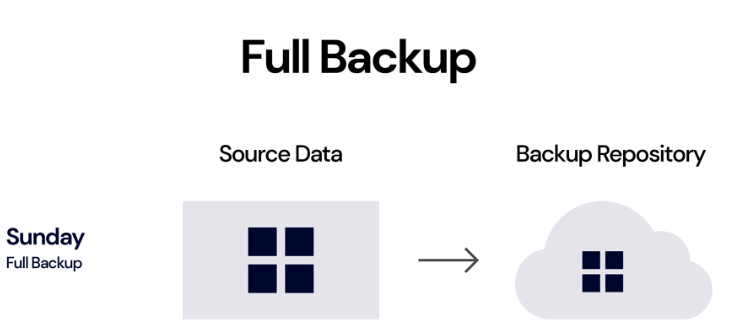
\includegraphics[width=\textwidth]{img/fullb.png}  
    \caption{Representatie van een full back-up \autocite{Rivas2022}}   
    \label{fig:fullback-up}           
\end{figure}
Een full back-up is een back-upmethode waarbij alle gegevens van een systeem op een specifiek moment volledig worden gekopieerd en opgeslagen. Dit betekent dat elk bestand zonder uitzonderingen wordt gekopieerd, zodat er een exacte kopie van de volledige dataset ontstaat \autocite{Beard2018}. Wanneer er zich een probleem voordoet, zoals het falen van een harde schijf, kan het hele bestandssysteem vanaf deze back-up volledig worden hersteld op een nieuwe schijf. Daarnaast kunnen ook individuele bestanden die verloren zijn gegaan, gemakkelijk worden teruggehaald uit de back-up. Dit soort back-up zorgt ervoor dat alle gegevens veilig zijn opgeslagen \autocite{Chervenak1998}. Full back-ups vormen vaak de basis van een back-upstrategie en worden regelmatig uitgevoerd om ervoor te zorgen dat alle gegevens volledig hersteld kunnen worden. Het concept en de implementatie van een full back-up is relatief eenvoudig omdat alle gegevens op één locatie zijn opgeslagen. Aan de andere kant is er het probleem van opslagcapaciteit. Stel bijvoorbeeld dat een bedrijf elke nacht een full back-up maakt van zijn servers naar een cloudopslagdienst, waarbij per keer 500 GB aan data wordt opgeslagen. Na een week is er al 3,5 terabyte aan gegevens in de cloud opgeslagen. Aangezien cloudproviders vaak kosten in rekening brengen op basis van gebruikte opslagcapaciteit en dataverkeer, kan dit snel leiden tot aanzienlijke maandelijkse kosten. Bedrijven met een beperkt IT-budget kunnen hierdoor in de problemen komen of worden gedwongen om strenger te selecteren welke gegevens ze precies opslaan in de back-up, omdat de opslagkosten oplopen naarmate de hoeveelheid opgeslagen data toeneemt. Daarbij kan het proces zelf ook veel tijd innemen. Dit kan voor problemen zorgen bij bedrijven waarbij de systemen aan moeten blijven. Vaak worden full back-ups gecombineerd met andere back-upmethodes. Daarnaast kost een full back-up veel tijd, wat een uitdaging kan zijn in omgevingen waar snelle gegevensbeschikbaarheid nodig is. Stel bijvoorbeeld dat een groot bedrijf tijdens kantooruren een full back-up wil maken van alle gegevens. Omdat deze back-up meerdere uren in beslag kan nemen, worden de systemen gedurende die tijd zwaar belast. Dit kan ertoe leiden dat andere processen vertraging oplopen of dat de server tijdelijk minder goed beschikbaar is voor werknemers die ook van die systemen afhankelijk zijn voor hun dagelijkse taken. Vanwege deze nadelen is het vaak beter om full back-ups aan te vullen met andere methoden \autocite{Nelson2011}.









\subsubsection{Incrementele back-up}
\begin{figure}[h] 
    \centering
    \captionsetup{justification=centering}
    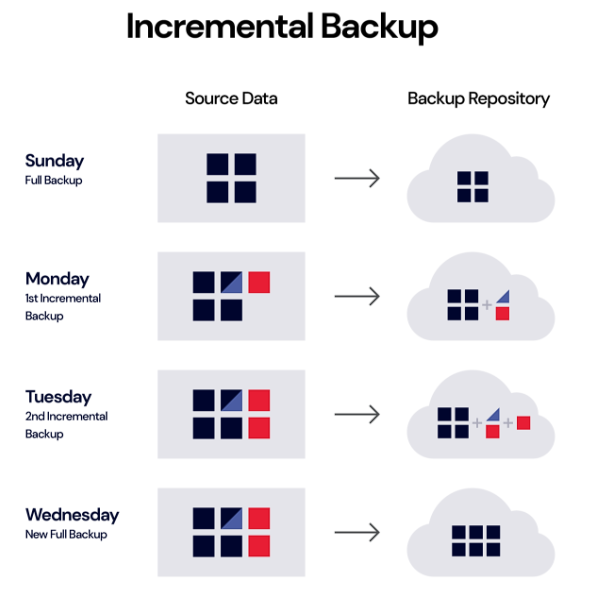
\includegraphics[width=0.5\textwidth]{img/incrementb.png}  
    \caption{Representatie van een incremental back-up \autocite{Rivas2022}}   
    \label{fig:incrback-up}           
\end{figure}

Een incrementele back-upstrategie houdt in dat na een initiële full back-up slechts de gegevens worden opgeslagen die sinds de laatste back-up zijn gewijzigd \autocite{Zhao2024}. Dit betekent dat een incrementele back-up alleen de veranderingen in de bestanden opneemt, in plaats van telkens een volledige kopie te maken van alle gegevens. Dit is vooral handig voor bedrijven die relatief vaak back-ups moeten maken, maar de opslag- en tijdskosten van een full back-up willen vermijden. Bijvoorbeeld, stel dat een bedrijf op maandag een full back-up uitvoert met al hun gegevens. Op dinsdag doet het bedrijf een incrementele back-up, waarbij enkel de wijzigingen sinds maandag worden opgeslagen. Dit gaat elke dag zo verder, elke dag wordt enkel de nieuwe of gewijzigde data opgeslagen ten opzichte van de dag ervoor. Omdat bedrijven steeds meer data beheren, biedt deze methode een efficiënte manier om opslagkosten te beperken, vooral wanneer gebruik wordt gemaakt van een cloudservice. Stel dat een bedrijf dagelijks slechts 1\% van zijn gegevens wijzigt; in plaats van elke dag een volledige kopie van bijvoorbeeld 1 TB te maken, slaat een incrementele back-up slechts de nieuwe 1\% op, wat 990 GB aan opslagruimte per dag bespaart. Dit maakt incrementele back-ups heel aantrekkelijk voor bedrijven die grote hoeveelheden data verwerken en frequente back-ups willen uitvoeren. Naast de besparing op opslagcapaciteit, zorgen incrementele back-ups voor kortere back-uptijden omdat alleen de gewijzigde bestanden worden opgeslagen. Dit betekent dat bedrijven vaker back-ups kunnen uitvoeren zonder hun systemen te vertragen. Een mediabedrijf dat met grote bestanden werkt, kan hierdoor bijvoorbeeld elk uur een incrementele back-up maken, in plaats van dagelijks een volledige back-up. Dit minimaliseert het risico op dataverlies, omdat in het geval van een storing, slechts maximaal een uur aan data verloren gaat in plaats van een hele dag. Hoewel incrementele back-ups voordelen bieden op het gebied van opslag en back-uptijden, brengen ze ook nadelen met zich mee, zoals langere hersteltijden\autocite{Chervenak1998}. Om een systeem te herstellen, heb je de laatste volledige back-up en alle volgende incrementele back-ups nodig en dit kan veel tijd kosten. Een financiële instelling die bijvoorbeeld op vrijdag een een systeemherstel moet uitvoeren, zal de volledige back-up van maandag plus alle incrementele back-ups tot en met donderdag moeten doorlopen. Dit kan relatief lang duren, wat leidt tot langere downtime, vooral in een noodsituatie waarin snelle hersteltijd van belang is. Een ander nadeel is de complexiteit van het beheer. Elke incrementele back-up hangt af van de vorige, wat betekent dat een fout in één back-up de hele herstelketen kan verstoren. Een IT-bedrijf dat dagelijks incrementele back-ups maakt, kan bijvoorbeeld problemen ondervinden als de back-up van woensdag beschadigd blijkt te zijn. Alle latere back-ups zijn afhankelijk van die ene back-up, wat het herstelproces moeilijker maakt. Dit vraagt om extra monitoring en beheer, zodat eventuele beschadigingen of herstelproblemen tijdig kunnen worden opgemerkt en opgelost.
\subsubsection{On-premise back-ups}
\subsubsection{Cloud back-ups}
\subsubsection{Offline back-ups}
\subsubsection{Immutable storage}
\subsection{Ransomware-resistente back-upoplossingen}
\subsection{Back-upmethoden en -technieken}
\subsection{Back-upmethoden en -technieken}
\subsection{Proof of Concept}